\subsection{Statechart Diagrams}


\textbf{Request State Diagram} \\
This state diagram shows the three states of a Reuquest: the Request is always created ad Reserved and then he can pass into the Started state or into the Finished one, depending on whether he arrives at the supermarket.

\begin{figure}[H] 
\centerline{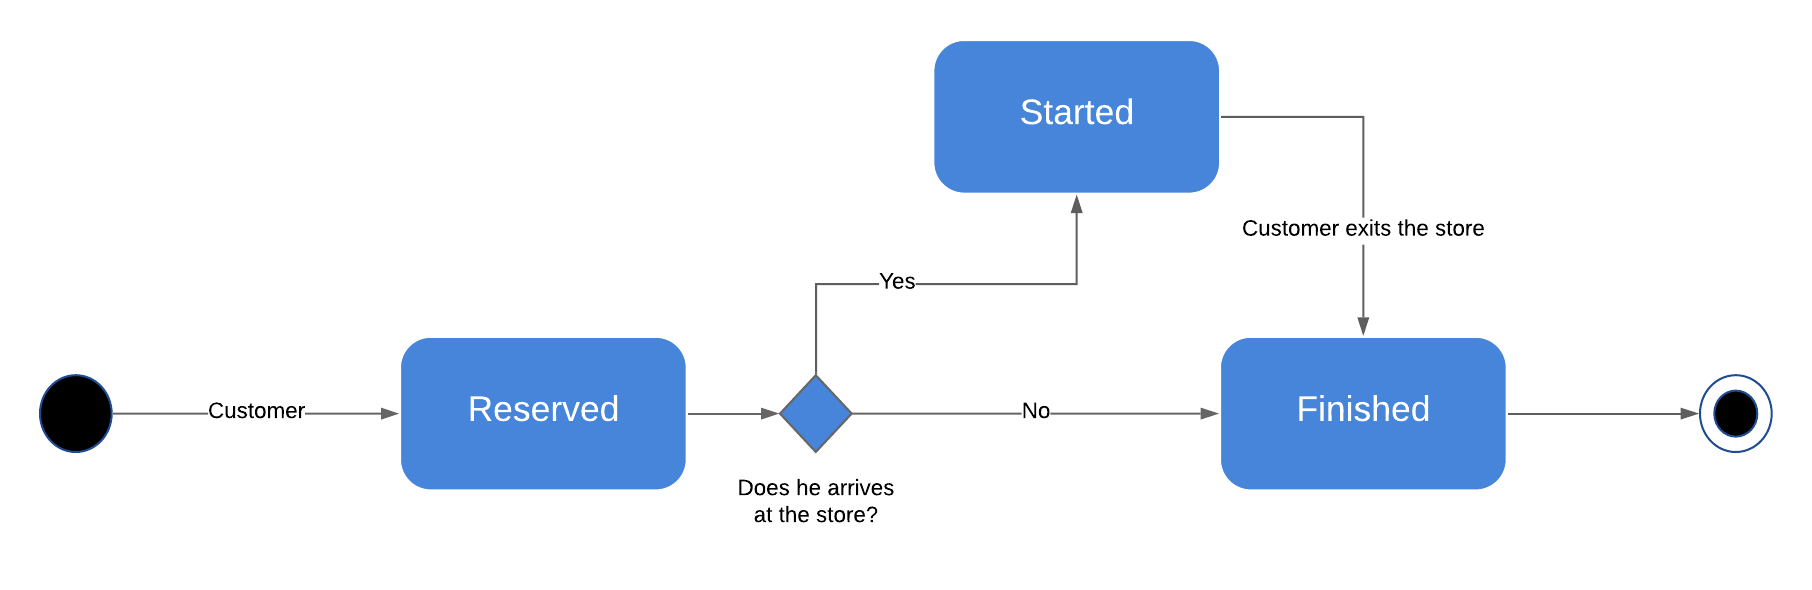
\includegraphics[scale=0.57]{RequestStateDiagram}}
\caption{Request State Diagram}
\end{figure}



\textbf{Ticket Entrance State Diagram}
This state diagram shows the different state of the entrance of a NoTechCustomer: when he arrives at the market, he is Reported by the StoreManager. If the supermarket is not full he can enter immediately the supermarket; otherwise, he has to wait for his waiting time.
\begin{figure}[H] 
\centerline{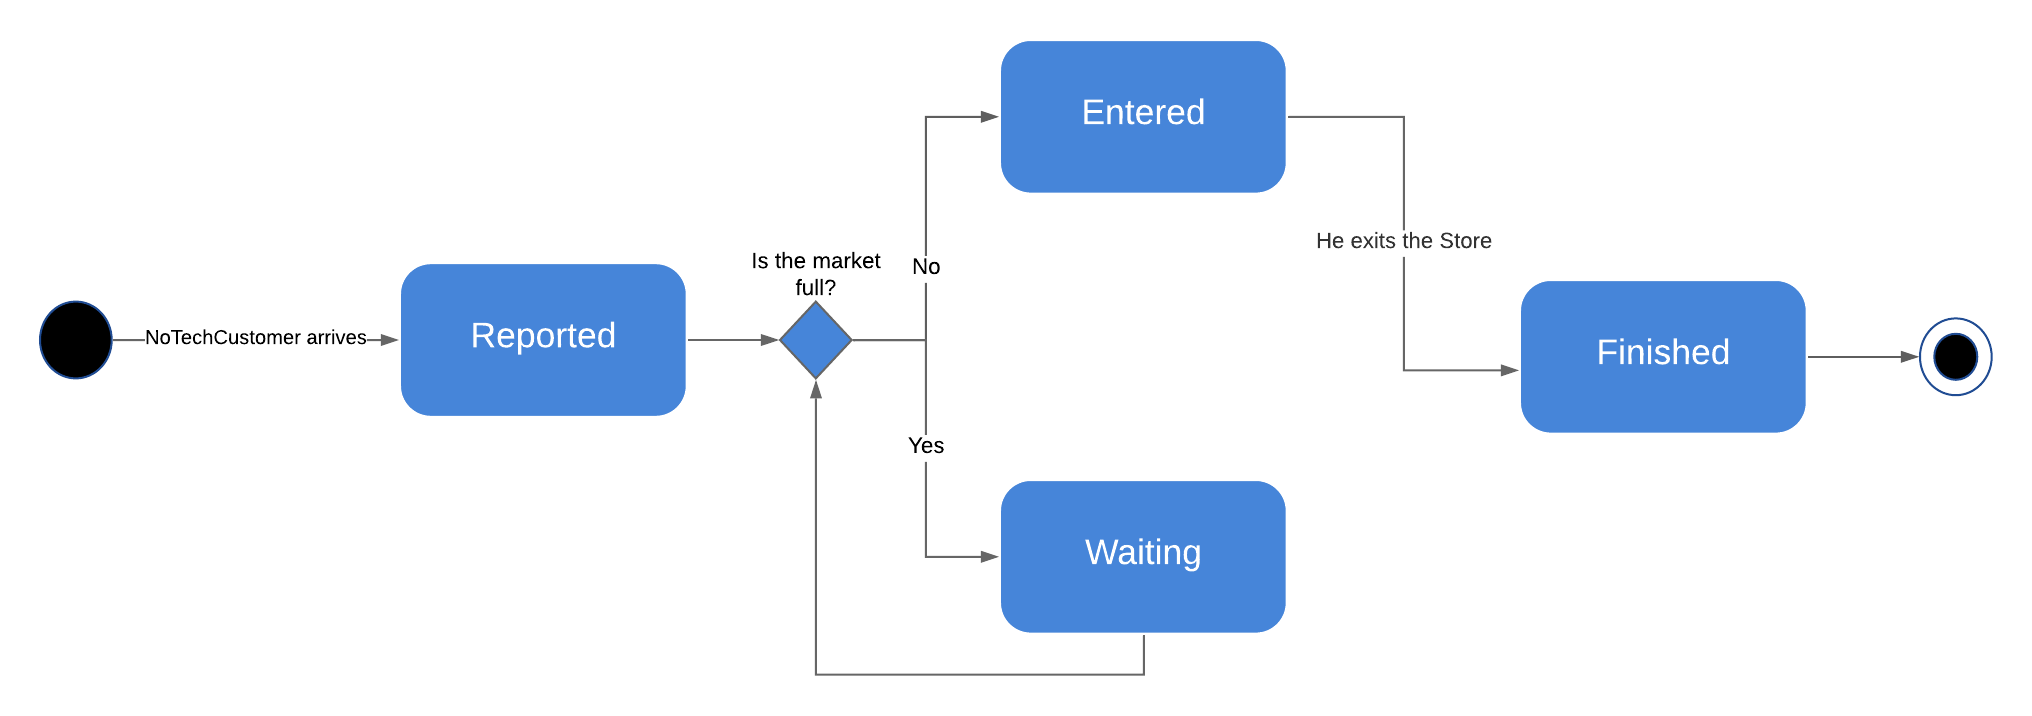
\includegraphics[scale=0.57]{TicketStateDiagram}}
\caption{Ticket Entrance State Diagram}
\end{figure}
 



 
 